\section{Congruence subgroups}
\label{sec:congruence-subgroups}

Let $N\geq 1$ be an integer. In this section we will consider subgroups of $\SL_2(\ZZ)$ that are especially nice to work with. There are other subgroups that are interesting but beyond the scope of this course.
\begin{definition}
  The \emphh{principal congruence subgroup} of level $N$ is
\[
\Gamma(N)=\{ \gamma\in\SL_2(\ZZ)~|~ \gamma\equiv \smtx 1001 \pmod{N}\}.
\]
\end{definition}

Note that $\Gamma(1)=\SL_2(\ZZ)$, so we are strictly generalizing Chapter~\ref{chap:modforms-full-level}. Note also that $\Gamma_0(N)$ can be defined as the kernel of the group homomorphism induced by the reduction map $\ZZ\to \ZZ/N\ZZ$:
\[
\pi_N\colon \SL_2(\ZZ)\to \SL_2(\ZZ/N\ZZ).
\]
Therefore, $\Gamma(N)$ is a normal subgroup of $\SL_2(\ZZ)$, of finite index.
\begin{proposition}
  The map $\pi_N$ is surjective.
\end{proposition}
\begin{proof}
  Exercise.
\end{proof}
There are too few principal congruence subgroups (only one for each $N\geq 1$), so it is desirable to consider more general subgroups.
\begin{definition}
  A subgroup $\Gamma\subseteq \SL_2(\ZZ)$ is a \emphh{congruence subgroup} if there is some $N\geq 1$ such that
\[
\Gamma(N)\subseteq \Gamma \subseteq \SL_2(\ZZ).
\]
The \emphh{level} of a congruence subgroup $\Gamma$ is the minimum $N$ such that $\Gamma(N)\subseteq \Gamma$.
\end{definition}

One can think of many different ways to construct congruence subgroups. There are two families that arise so frequently that have special notation for them:

\begin{example}
For each $N\geq 1$, define
  \[
\Gamma_1(N)=\{\smtx{1}{*}{0}{1}\pmod N\},
\]
and also
  \[
\Gamma_0(N)=\{\smtx{*}{*}{0}{*}\pmod N\}.
\]
\end{example}

\begin{lemma}
  For each $N\geq 1$ there are inclusions
$\Gamma(N) \subseteq \Gamma_1(N) \subseteq \Gamma_0(N) \subseteq \SL_2(\ZZ)$,
and
\[
[\Gamma_1(N)\colon \Gamma(N)] = N,\quad [\Gamma_0(N)\colon \Gamma_1(N)] = N\prod_{p\mid N} \left(1-\frac 1p\right),\quad [\SL_2(\ZZ)\colon \Gamma_0(N)] = N\prod_{p\mid N} \left(1+\frac 1p\right).
\]
\end{lemma}
\begin{proof}
  Exercise.
\end{proof}

\begin{remark}
  The inclusions are strict except for $N=1$ (where all groups coincide) and for $\Gamma_0(2)=\Gamma_1(2)$.
\end{remark}

%Recall the slash operator introduced in Section~\ref{sec:upper-half-plane}.
\begin{definition}
  A function $f\colon\HH\to\CC$ is \emphh{weakly modular} of weight $k$ with respect to $\Gamma$ if it is meromorphic on $\HH$ and it satisfies
\[
f|_k\gamma = f,\quad \forall \gamma\in\Gamma.
\]
\end{definition}
\newcommand{\Cusps}{\operatorname{Cusps}}
\section{Cusps}
\label{sec:cusps}

Of course we will need to understand fundamental domains for the action of congruence subgroups on $\HH$. Here is for example a fundamental domain for $\Gamma_0(2)$:
\begin{figure}[h]
  \centering
  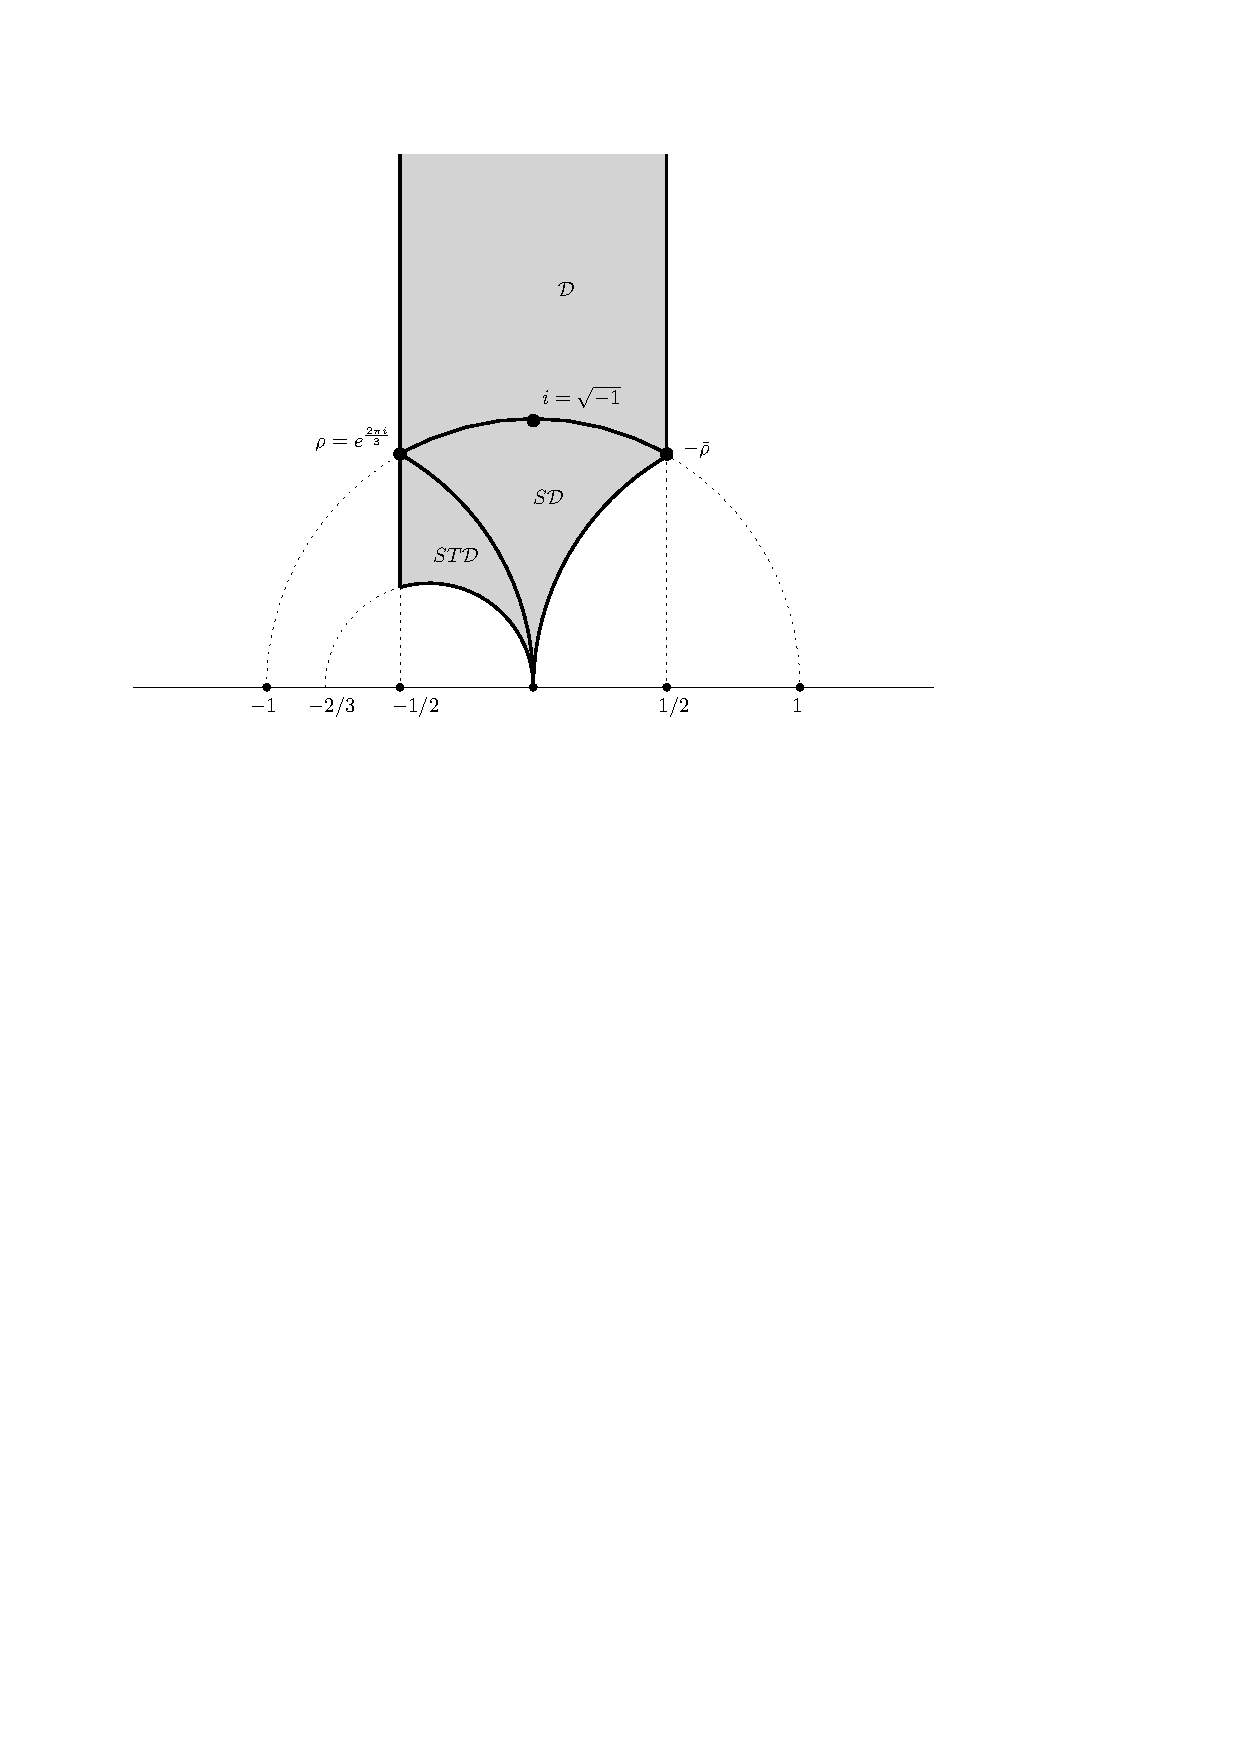
\includegraphics{fundomGamma02.pdf}
  \caption{A fundamental domain for $\Gamma_0(2)$}
  \label{fig:fundom-gamma02}
\end{figure}

In this case, the fundamental domain contains two points in its closure which do not belong to $\HH$: the cusp $\infty$ as before, but also $0$. The following result gives a construction of a fundamental domain for any congruence subgroup, using translates of the fundamental domain $\cD$ of $\SL_2(\ZZ)$ seen in Chapter~\ref{ch:modforms-full-level}.
\begin{proposition}
  Let $\Gamma$ be a congruence subgroup of $\SL_2(\ZZ)$. If there is a decomposition
\[
\Gamma\backslash \SL_2(\ZZ)=\bigcup_{h\in R} \Gamma h,\quad R\text{ finite,}
\]
then the set $\cD_\Gamma=\cup_{h\in R} h\cD$ is a (possibly non-connected) fundamental domain for $\Gamma$.
\end{proposition}
\begin{proof}
  If $z\in\HH$, then there exists $g\in\SL_2(\ZZ)$ and $z_0\in\cD$ such that $z = gz_0$. The coset decomposition implies that there is some $\gamma\in R$ and some $h\in \Gamma$ such that $g=h\gamma$. Therefore
\[
z = h\gamma z_0.
\]
Since $z_0'=\gamma z_0\in \gamma\cD\subset \cD_\Gamma$ we have written $z=h z_0'$ with $h\in\Gamma$.

It remains to be shown that if $z\in\stackrel{\circ}{\cD_\Gamma}$ and $\gamma z \in\stackrel{\circ}{\cD_\Gamma}$ for some $\gamma\in\Gamma$, then $\gamma = 1$. For that, let $\eps>0$ be small enough so that the ball $B_\eps(z)$ of radius $\eps$ around $z$ is fully contained in $\stackrel{\circ}{\cD_\Gamma}$. The ball $B_\eps(z)$ intersects some translates of $\cD$, say:
\[
B_\eps(z)\cap h\cD \neq \emptyset\iff h\in R'\subseteq R.
\]
Consider the translated ball $\gamma B_\eps(z)=B_\eps(\gamma z)$. Since $\gamma z$ is also in the interior of $\cD_\Gamma$, we deduce that $\gamma B_\eps(z)$ must intersect the interior of some translate of $\cD$, say $h\stackrel{\circ}{\cD}$, for some $h\in R$. Therefore:
\[
\gamma B_\eps(z)\cap h\stackrel{\circ}{\cD}\neq \emptyset \implies B_\eps(z)\cap \gamma^{-1}h\stackrel{\circ}{\cD}\neq \emptyset.
\]
Since we listed all the translates whose interior intersected with $B_\eps(z)$, we must have that $\gamma^{-1}h = h_0$. But now $\Gamma h = \Gamma \gamma^{-1}h = \Gamma h_0$, and since both $h$ and $h_0$ belong to $R$, we must have $h=h_0$. Therefore $\gamma^{-1}=1$, or $\gamma=1$ as we wanted.
\end{proof}

In order to further study the cusps, we consider the \emphh{rational projective line} $\PP^1(\QQ)=\QQ \cup\{\infty\}$. Note that $\SL_2(\ZZ)$ (in fact $\GL_2(\QQ)$) acts on $\PP^1(\QQ)$ by fractional linear transformations:
\[
\gamma x = \frac{ax +b}{cx+d},\quad \gamma = \mtx abcd\in\SL_2(\ZZ),x\in\PP^1(\QQ).
\]
Here we understand that $\gamma\infty = \frac ac$, and $\gamma x = \infty$ if $cx = -d$.

\begin{proposition}
  The action of $\SL_2(\ZZ)$ on $\PP^1(\QQ)$ is transitive, and it induces a bijection
\[
\SL_2(\ZZ)/\SL_2(\ZZ)_\infty\cong \PP^1(\QQ),\quad \SL_2(\ZZ)_\infty = \langle \pm T\rangle.
\]
\end{proposition}
\begin{proof}
  We will see that the orbit of $\infty$ is all of $\PP^1(\QQ)$, where we note that $\smtx abcd \infty = \frac ac$. Given $\frac ac\in\PP^1(\QQ)$ in reduced terms (that is, such that $(a,c)=1$), then B\'ezout's identity asserts the
existence of integers $b$ and $d$ such that $ad-bc=1$. Then the matrix $\smtx abcd$ belongs to $\SL_2(\ZZ)$ and takes $\infty$ to $\frac ac$.

The stabilizer of $\infty$, written $\SL_2(\ZZ)_\infty$, is:
\[
\SL_2(\ZZ)_\infty = \left\{\mtx abcd ~|~ \mtx abcd \infty = \infty\right\} = \left\{\mtx abcd ~|~ \frac ac = \infty\right\} = \left\{\mtx ab0d\right\} = \langle \pm T\rangle.
\]
\end{proof}

\begin{definition}
  The set of \emphh{cusps} of a congruence subgroup $\Gamma$ is the set $\Cusps(\Gamma)$ of $\Gamma$-orbits of $\PP^1(\QQ)$. Equivalently,
\[
\Cusps(\Gamma) = \Gamma\backslash \SL_2(\ZZ) / \SL_2(\ZZ)_\infty.
\]
\end{definition}

If $P = [\frac ac]$ is a cusp of $\Gamma$, set $\Gamma_P$ for the \emphh{stabilizer} of $P$ in $\Gamma$, the elements of $\Gamma$ fixing $P$.
\begin{lemma}
  If $\gamma_P(\infty) = P$, then
\[
\Gamma_P = \Gamma\cap \gamma_P\SL_2(\ZZ)_\infty \gamma_P^{-1}.
\]
\end{lemma}
\begin{proof}
 Let $\gamma\in\Gamma$. Then observe that
\begin{align*}
\gamma\in\Gamma_P&\iff \gamma P = P\iff \gamma \gamma_P\infty=\gamma_P\infty\\
&\iff \gamma_P^{-1}\gamma\gamma_P\infty=\infty\\
&\iff \gamma_P^{-1}\gamma\gamma_P\in \SL_2(\ZZ)_\infty\\
&\iff \gamma\in \gamma_P\SL_2(\ZZ)_\infty \gamma_P^{-1}.
\end{align*}
This concludes the proof.
\end{proof}

\begin{lemma}
The subgroup $H_P = \gamma_P^{-1}\Gamma\gamma_P\cap \SL_2(\ZZ)_\infty \subseteq \SL_2(\ZZ)_\infty$
does not depend on the choice of the representative for $P$, and has finite index in $\SL_2(\ZZ)_\infty$.
\end{lemma}
\begin{proof}
  Just note that if $\frac{a'}{c'}$ is another representative for $P$, then $\gamma_P$ gets modified into $\gamma\gamma_P$ for some $\gamma\in\Gamma$. Then $(\gamma\gamma_P)^{-1}\Gamma(\gamma\gamma_P) = \gamma_P^{-1}\Gamma\gamma_P$.
\end{proof}

\begin{lemma}
  Let $H$ be a subgroup of finite index in $\SL_2(\ZZ)_\infty$, and let $h$ be the index of $\{\pm 1\}H$ in $\SL_2(\ZZ)_\infty$. Then $H$ is one of he following:
\[
H = \begin{cases}
\langle \smtx 1h01\rangle&\\
\langle \smtx{-1}{h}{0}{-1}\rangle&\\
\{\pm 1\}\times \langle \smtx 1h01\rangle&
\end{cases}
\]
\end{lemma}
\begin{proof}
  Exercise.
\end{proof}
\begin{definition}
The integer $h_\Gamma(P)=h$ in the above lemma is called \emphh{width of a cusp} $P$ for $\Gamma$. A cusp is an \emphh{irregular cusp} if $\gamma_P^{-1}\Gamma_P\gamma_P$ is of the form $\langle \smtx{-1}{h}{0}{-1}\rangle$, and it is \emphh{regular cusp} otherwise.
\end{definition}

\begin{example}
  In this example we show that if $p$ is any prime, then $\Cusps(\Gamma_0(p)) = \{ \infty, 0\}$.

Write an element $\gamma\in\Gamma_0(p)$ as $\smtx{a}{b}{pc}{d}$, with $a,b,c,d\in\ZZ$ satisfying $ad-pbc =1$. The orbit of $\infty$ is:
\[
\Gamma_0(p)\cdot \infty = \left\{\mtx{a}{b}{pc}{d}\infty\right\} = \left\{\frac{a}{pc}~\colon~ a,c\in\ZZ,\gcd(a,pc) = 1\right\} = \left\{ \frac{r}{s}~\colon~ p\mid s, \gcd(r,s)=1\right\}.
\]
We thus see the orbit of the cusp $\infty$ consists of infinity together with all the rationals which when expressed in reduced terms have a denominator which is divisible by $p$. One element which is not in this orbit is $0=\frac{0}{1}$. Let us study then the orbit of $0$.
\[
\Gamma_0(p) \cdot 0 = \{\mtx{a}{b}{pc}{d} 0\} = \{\frac{b}{d}~\colon~ b,d\in\ZZ, \gcd(b,d)=1, p\nmid d\}.
\]
\end{example}
As we have seen in the example above, each cusp may have a different width. However, if $\Gamma$ is a normal congruence subgroup of $\SL_2(\ZZ)$, the subgroup $H_P$ does not depend on the cusp $P$ and hence all cusps have the same width and regularity.

Although one can have more cusps than the index of $\Gamma$, the last result of this section says that this is basically right, once one counts in a proper way. To prove it, we will need a group-theoretic result.

\begin{lemma}[orbit--stabilizer for infinite groups]
  \label{lemma:orbit-stabilizer}
Let $G$ be a group acting transitively on a set $X$ and let $H$ be a finite index subgroup of $G$. Then for any $x\in X$ the stabilizer of $x$ in $H$ has finite index in the stabilizer of $x$ in $G$, and the following formula holds:
\[
\sum_{x\in H\backslash X} [G_x\colon H_x]=[G\colon H].
\]
\end{lemma}
\begin{proof}
  Let $x\in X$, and consider the inclusion map $G_x\to G$. By taking the quotient by $H$ we get $G_x\to H\backslash G$. Suppose $g_1, g_2$ are mapped to the same element $Hg$ in $H\backslash G$. This means that $Hg_1 = Hg_2$, or that $g_2g_1^{-1}$ belongs to $H$. Since $g_2g_1^{-1}$ stabilizes $x$ as well, we deduce that $H_x g_1 = H_x g_2$. Therefore there is an injection of $H_x\backslash G_x\injects H\backslash G$. Since by assumption the latter set is finite, so is the first. Note also that the image of the map is precisely $H\backslash HG_x$, and thus we also obtain $[G_x\colon H_x] = [H G_x\colon H]$.

To prove the second assertion, fix an element $x_0\in X$, and consider the map
\[
H\backslash G\tto H\backslash X,\quad Hg\mapsto Hgx_0
\]
which is surjective because $G$ acts transitively on $X$. The fibre $T_{Hx}$ of an orbit $Hx$ consists of the set of classes $Hg$ such that $Hgx_0 = Hx$. Let $g_x\in G$ be such that $g_x x_0 = x$. Write $Hg = Hg'g_x$ and then we have:
\begin{align*}
T_{Hx}&\cong \{Hg'\in H\backslash G\colon Hg'g_xx_0 = Hx\} = \{Hg'\in H\backslash G\colon Hg'x=Hx\}= H\backslash(H G_x)\cong H_x\backslash G_x.
\end{align*}
This allows us to find a formula for $[G\colon H]$:
\begin{align*}
[G\colon H]&=\# (H\backslash G) = \sum_{x\in R} \# T_{Hx} = \sum_{x\in R} [G_x\colon H_x].
\end{align*}
\end{proof}

\begin{theorem}
  Let $\Gamma$ be a congruence subgroup. Then we have
\[
\sum_{P\in \Cusps(\Gamma)} h_\Gamma(P) = [\SL_2(\ZZ)\colon \{\pm 1\}\Gamma].
\]
\end{theorem}
\begin{proof}
  Consider the group $G=\PSL_2(\ZZ)=\SL_2(\ZZ)/\{\pm 1\}$, which acts transitively on the set $X=\PP^1(\QQ)$. Let $H$ be the image of $\Gamma$ in $G$. Note that $H\backslash X=\Cusps(\Gamma)$. Also, $G_\infty$ is the image in $G$ of $\SL_2(\ZZ)_\infty$. For each $x\in X$, let $\gamma\in G$ be such that $\gamma \infty = x$. Then
\[
G_x=\gamma G_\infty\gamma^{-1},\text{ and}\quad H_x= \gamma \left(\gamma^{-1}H\gamma\right)_\infty \gamma^{-1}.
\]
Therefore
\[
[G_x\colon H_x] = [\bar\SL_2(\ZZ)\colon \bar \Gamma_P] = h_\Gamma(P),
\]
where by $\ol{(\cdot)}$ we write the image of the group inside $G$. Then applying Lemma~\ref{lemma:orbit-stabilizer} to this setting gives
\[
\sum_{P\in \Cusps(\Gamma)} h_\Gamma(P) = [G\colon H] = [\SL_2(\ZZ)\colon \{\pm 1\}\Gamma].
\]
\end{proof}
\section{Fourier expansion at infinity}
\label{sec:fourier-expansion-at-infinity}

Let $\Gamma$ be a congruence subgroup of level $N$. Note that the matrix $\smtx 1N01$ belongs to $\Gamma(N)$, and thus there is a minimum $h>0$ with the property that $\smtx 1h01 \in\Gamma$.
\begin{definition}
  The \emphh{fan width} of $\Gamma$ is the minimum $h>0$ such that $\smtx 1h01\in\Gamma$.
\end{definition}
\begin{remark}
  The fan width of a congruence subgroup of level $N$ is a divisor of $N$.
\end{remark}
Write
\[
q_h =q_h(z)= e^{\frac{2\pi i z}{h}},
\]
and note that $z\mapsto q_h(z)$ is periodic with period $h$. Define $g$ by $g = f\circ q_h^{-1}$.
That is, $g(q_h) = f(z)$. Although $q_h$ is not invertible, the above definition makes sense, and $g$ has
a Laurent expansion.
\begin{definition}
  The $q$-expansion of $f$ at infinity is the Laurent expansion:
\[
f(z) = g(q_h)=\sum_{n=-\infty}^\infty a(n)q_h^n.
\]
\end{definition}

\section{Expansions at cusps}
\label{sec:expansions-at-cusps}


Let $s$ be a cusp, $s\neq \infty$. Write $s =\alpha\infty$ for some $\alpha\in\SL_2(\ZZ)$, and consider the equation:
\[
f(\alpha z) = j(\alpha,z)^{k}(f|_k\alpha)(z).
\]
 Since $j(\alpha,z)\neq 0,\infty$ when $z$ is near $\infty$, the behavior of $f(z)$ near $s$  is related to the behavior of $(f|_k\alpha)(z)$ near $\infty$. Assume that $f$ is weakly modular for the congruence subgroup $\Gamma$. Since\[
(f|_k\alpha)|_k(\alpha^{-1}\gamma\alpha) = (f|_k\gamma)|_k\alpha = f|_k\alpha,
\]
the new function $f|_k\alpha$ is invariant under the group $\Gamma'=\alpha^{-1}\Gamma\alpha$. Since $\Gamma(N)$ is normal inside $\SL_2(\ZZ)$, we deduce that $\Gamma'$ is also a congruence subgroup of level $N$. Hence $f|_k\alpha$ has a Fourier expansion at infinity as in Section~\ref{sec:fourier-expansion-at-infinity} in powers of $q_N$.
\begin{definition}
  The \emphh{expansion of $f$ at a cusp} $s$ is the expansion:
\[
f|_k\alpha = \sum_{n=-\infty}^\infty b(n)q_N^n.
\]
\end{definition}

\section{Definition of modular forms}
The expansions at different cusps allow us to define modular forms for arbitrary congruence subgroups.
\begin{definition}
\label{def:modforms-congruence}
  A function $f\colon\HH\to\CC$ is a \emphh{modular form} of weight $k$ for a congruence subgroup $\Gamma$ if:
  \begin{enumerate}
  \item $f$ is holomorphic on $\HH$,
  \item $f|_k\gamma = f$ for all $\gamma\in\Gamma$, and
  \item $f|_k\alpha$ is holomorphic at infinity for all $\alpha\in\SL_2(\ZZ)$.
  \end{enumerate}
 A function is a \emphh{cusp form} of weight $k$ for a congruence subgroup $\Gamma$ if instead of $3$ is satisfies:
 \begin{enumerate}[resume]
\item[3'.] $f|_k\alpha$ vanishes at infinity for all $\alpha\in\SL_2(\ZZ)$.
 \end{enumerate}
The \emphh{space of modular forms} of weight $k$ for a congruence subgroup $\Gamma$ is written $M_k(\Gamma)$; the \emphh{space of cusp forms} of weight $k$ for a congruence subgroup $\Gamma$ is written $S_k(\Gamma)$.
\end{definition}
\begin{proposition}
  Suppose that $f\colon\HH\to\CC$ satisfies $1$ and $2$ above. Suppose that $f$ is holomorphic at infinity. That is,
\[
f(z) = \sum_{n=0}^\infty a(n)q_N^n.
\]
Furthermore, suppose that there exists constants $C>0$ and $r>0$ such that:
\[
|a(n)|< Cn^r,\quad \forall n > 0.
\]
Then $f$ satisfies $3$, and thus $f\in M_k(\Gamma)$.
\end{proposition}
\begin{proof}
  Exercise.
\end{proof}
\begin{remark}
  In fact, the converse is also true: if the Fourier coefficients of $f$ grow as $Cn^r$ as above, then condition $3$ in Definition~\ref{def:modforms-congruence} is satisfied. The proof of this fact uses Eisenstein series for congruence subgroups, and thus will be postponed until we introduce those.
\end{remark}

\begin{example}
  Let $f$ be a weakly-modular form of weight $k$ for the full modular subgroup. Consider the function $g(z) = f(Nz)$. If $\gamma\in\Gamma_0(N)$ is of the form $\gamma=\smtx abcd$, then since $N\mid c$ the matrix
\[
\gamma'=\mtx a{bN}{c/N}{d}
\]
is in $\SL_2(\ZZ)$. Therefore we may compute:
\begin{align*}
g(\gamma z) &= f(N(\gamma z)) = f(\frac{Naz+bN}{cz+d}) \\
&= f(\frac{a(Nz)+bN}{c/N (Nz) + d}) = f(\gamma'(Nz))\\
&=(c/N(Nz) + d)^{k}f(Nz) = j(\gamma,z)^k g(z).
\end{align*}
Therefore the function $g$ is weakly-modular of weight $k$ for the congruence subgroup $\Gamma_0(N)$. In fact, this operation defines injections
\[
M_k(\SL_2(\ZZ))\to M_k(\Gamma_0(N))
\]
which will play an important role later in the course, in the Atkin-Lehner-Li theory of old/new forms.
\end{example}

We end this section by realizing that the definition of modular forms can be checked by finitely many computations. Suppose that $\sigma=\alpha\infty$ and $\tau=\beta\infty$ are two cusps (here $\alpha$ and $\beta$ are in $\SL_2(\ZZ)$). Suppose that $\sigma=\gamma\tau$ with $\gamma\in\Gamma$.
\begin{proposition}
If
\[
f|_k\alpha = \sum_{n=-\infty}^\infty a(n)q_h^n,
\]
then
\[  f|_k\beta = \sum_{n=-\infty}^\infty b(n)q_h^n,\quad b(n) = (\pm 1)^k e^{\frac{2\pi i n j}{h}} a(n), j\in \ZZ.
\]
\end{proposition}
\begin{proof}
  By assumption $\alpha\infty=\gamma\beta\infty$, so $\alpha^{-1}\gamma\beta\infty=\infty$, and therefore since the only matrices that fix infinity are of the form $\pm \smtx 1j01$ we have:
\[
\alpha^{-1}\gamma\beta = \pm\mtx 1j01,\quad j\in\ZZ.
\]
This means that
\[
\beta = \pm \gamma^{-1}\alpha\mtx 1j01,
\]
and therefore:
\begin{align}
f|_k\beta &= f|_k\pm I |_k \gamma^{-1} |_k\alpha |_k \mtx 1j01 = (\pm 1)^k\sum a(n)e^{\frac{2\pi i n z}{h}} |_k \mtx 1j01\\
&=(\pm 1)^k\sum a(n) e^{\frac{2\pi i n (z+j)}{h}}.
\end{align}
\end{proof}
\begin{corollary}
  For each $n\in\ZZ$, we have $a(n)=0$ if and only if $b(n)=0$. In particular, it is enough to check $3$ or $3'$ for one representative from each of the equivalence classes of cusps.
\end{corollary}

\section{Valence formula for congruence subgroups}

  Let $\Gamma$ be a congruence subgroup of level $N$. In order to state the next result we need to define the order of a weakly-modular function at a cusps $P\in\Cusps(\Gamma)$.
\begin{definition}
  Let $f$ be a weakly-modular form of weight $k$ for $\Gamma$, and let $P$ be a cusp of $\Gamma$ of width $h_\Gamma(P)$. Since $f(z+N)=f(z)$, we can write $f$ as a Laurent series in $q_N=e^{\frac{2\pi i z}{N}}$, say
\[
f(q_N) = \sum_{n\geq n_0} a_n q_N^n,\quad a_{n_0}\neq 0.
\]
The \emphh{order of vanishing} of $f$ at $P$ is $v_P(f) = \frac{h_\Gamma(P)}{N}n_0$.
\end{definition}

Here is a generalization of Theorem~\ref{thm:valence-formula} to arbitrary congruence subgroups.
\begin{theorem}[valence formula for congruence subgroups]
  Let $\Gamma$ be a congruence subgroup, and let $k$ be an integer. Let $f$ be a non-zero meromorphic function on $\HH\cup\{\infty\}$, which is weakly-modular of weight $k$ for $\Gamma$. Then we have
\[
\sum_{z\in\Gamma\backslash\HH} \frac{v_z(f)}{\#\ol\Gamma_z} +\sum_{P\in\Cusps(\Gamma)} v_P(f)=\frac{k}{12}[\PSL_2(\ZZ)\colon\ol\Gamma].
\]
\end{theorem}
\begin{proof}
  Write $d_\Gamma=[\PSL_2(\ZZ)\colon\ol\Gamma]$, let $R$ be a set of coset representatives for $\ol\Gamma\backslash\PSL_2(\ZZ)$, and define $F=\prod_{\gamma\in R} f|_k\gamma$. Note that $F$ is weakly-modular of weight $kd_\Gamma$ for $\SL_2(\ZZ)$, and it is meromorphic at $\infty$. By Theorem~\ref{thm:valence-formula} we have
\[
v_\infty(F)+\frac 12 v_i(F) + \frac 13 v_\rho(F) +\sum_{w\in W} v_w(F) = \frac{k}{12} d_\Gamma.
\]
Another way to write the above is:
\[
 v_\infty(F) + \sum_{z\in\PSL_2(\ZZ)\backslash\HH} \frac{v_z(F)}{\#\PSL_2(\ZZ)_z} = \frac{k}{12} d_\Gamma.
\]
We may now compute:
\begin{align*}
v_z(F) &= \sum_{\gamma\in\ol\Gamma\backslash\PSL_2(\ZZ)} v_z(f|_k\gamma) = \sum_{\gamma\in\ol\Gamma\backslash\PSL_2(\ZZ)} v_{\gamma z}(f)=\sum_{w\in\ol\Gamma\backslash \PSL_2(\ZZ)z} [\PSL_2(\ZZ)_w\colon\ol\Gamma_w] v_w(f).
\end{align*}
The last equality follows by grouping all elements $\gamma$ such that $\gamma z=w$, for each possible $w$. Now, since $\PSL_2(\ZZ)_w$ is finite and independent of $w\in \ol\Gamma\backslash\PSL_2(\ZZ)z$, we get
$[\PSL_2(\ZZ)_w\colon\ol\Gamma_w]=\frac{\# \PSL_2(\ZZ)_z}{\#\ol\Gamma_w}$.
Dividing by $\#\PSL_2(\ZZ)_z$ we obtain
\[
\frac{v_z(F)}{\#\PSL_2(\ZZ)_z} = \sum_{w\in \ol\Gamma\backslash \PSL_2(\ZZ)z} \frac{v_w(f)}{\#\ol\Gamma_w}.
\]
By summing over a set of representatives for $\PSL_2(\ZZ)\backslash \HH$ we finally obtain
\begin{align*}
\sum_{z\in\PSL_2(\ZZ)\backslash\HH} \frac{v_z(F)}{\#\PSL_2(\ZZ)_z} &=\sum_{z\in\PSL_2(\ZZ)\backslash \HH}\sum_{w\in\ol\Gamma\backslash \PSL_2(\ZZ)z} \frac{v_w(f)}{\#\ol\Gamma_w}=\sum_{w\in\ol\Gamma\backslash\HH} \frac{v_w(f)}{\#\ol\Gamma_w}.
\end{align*}
In order to conclude the proof it remains to be shown that $v_\infty(F) = \sum_{P\in\Cusps(\Gamma)} v_P(f)$. We first prove it assuming that $\ol \Gamma$ is normal in $\PSL_2(\ZZ)$. In this case, we have
\begin{align*}
d_\Gamma v_\infty(F) &= \sum_{P\in\Cusps(\Gamma)} h_\Gamma(P)v_\infty(F)\\
&=\sum_{P\in\Cusps(\Gamma)} v_P(F)\\
&=\sum_{P\in\Cusps(\Gamma)} \sum_{\gamma\in R} v_{\gamma P}(f)\\
&=\sum_{P\in\Cusps(\Gamma)} \sum_{P'\in\Cusps(\Gamma)} \#\{\gamma\in R ~|~ \gamma P = P'\} v_{P'}(f)\\
&=\sum_{P'\in\Cusps(\Gamma)} \sum_{P\in\Cusps(\Gamma)} \#\{\gamma\in R ~|~ \gamma P = P'\} v_{P'}(f)\\
&=d_\Gamma\sum_{P'\in\Cusps(\Gamma)} v_{P'}(f).
\end{align*}
Note that any congruence subgroup $\Gamma$ contains a subgroup (for instance $\Gamma(N)$) which is normal in $\SL_2(\ZZ)$, and such that it is of finite index. Therefore it is enough to show that, if $\Gamma'\subset \Gamma$ have finite index and $g$ is weakly modular of weight $k$ for $\Gamma$, then
\[
\sum_{P'\in \Cusps(\Gamma')} v_{P'}(f) = \frac{d_{\Gamma'}}{d_\Gamma} \sum_{P'\in \Cusps(\Gamma')} v_{P'}(f).
\]
Let $P\in\Cusps(\Gamma)$ and $P'\in\Cusps(\Gamma')$ be such that $[P]=[P']$ inside $\Cusps(\Gamma)$. Pick $\sigma\in\SL_2(\ZZ)$ such that $\sigma\infty = [P]$ in $\Cusps(\Gamma)$. Write also $n_0 = v_P^\Gamma(g)$, and $m = \frac{h_{\Gamma'}}{h_\Gamma}$. Then:
\[
(g|_k\sigma)(z) = \sum_{n\geq n_0} a_n(g) e^{\frac{2\pi i n z}{h_\Gamma}} = \sum_{n\geq n_0} a_n(g)e^{\frac{2\pi i nmz}{h_{\Gamma'}}} = \sum_{n\geq mn_0} a_n(g)e^{\frac{2\pi i nz}{h_{\Gamma'}}}.
\]
Hence we have $v_{P'}(g) = m v_P(g)$, as we wanted. This concludes the proof of the valence formula.
\end{proof}

As for level $1$, the valence formula gives a criterion for equality of modular forms:
\begin{corollary}
  Let $f$ and $g$ be two modular forms in $M_k(\Gamma)$, whose $q$-expansions (at one cusp of $\Gamma$) coincide up to the term $\frac{k}{12}[\PSL_2(\ZZ)\colon\ol\Gamma]$. Then $f$ and $g$ are equal.
\end{corollary}

There are dimension formulas for congruence subgroups (see~\cite[Chapter 3]{diamond-shurman}) but we will not see them in this course.


%%% Local Variables: 
%%% mode: latex
%%% TeX-master: "main"
%%% End: 
